\chapter{Fejlesztői dokumentáció}
\label{ch:impl}

A szoftver működésének részletezéséhez elengedhetetlen a membránrendszerek formális modelljének ismerete, hiszen ezen rendszerek sajátos viselkedése az architechturális kérdésekben döntő szerepet képez.

A teljes definíció előtt azonban érdemes még pár fogalmat bevezetni. Általánosan tehát egy olyan absztrakt számítási modell áll a szoftver központjában, amely egy biológiai sejthez hasonló felépítéssel rendelkezik, az egymásba ágyazott membránok régiókat különítenek el, amely régiókban különböző objektumok helyezkedhetnek el. A rendszerben az objektumokon felül szabályokat is rendelhetünk régiókhoz, ezen szabályok felelősek a membránrendszer állapotában végbemenő változásokért. A szabályokat a megfelelő feltételek teljesülése esetén kötelesek vagyunk alkalmazni, így egy evolúciós lépés a rendszer számításában addig tart, amíg van legalább egy akalmazható szabály. Érdemes már megjegyezni, hogy egy régió beazonosításához egy egyedi azonosítóra van szükség, illetve, hogy egy régiót könnyen azonosítani lehet az őt legszűkebben tartalmazó membránnal. Így természetes módon adódik, hogy a régiókat fa struktúrába tudjuk szervezni, amelyben minden egyes csúcs egy egyedi azonosítóval rendelkezik. Ezen fában a levelek az elemi membránokat reprezentálják, azaz azokat a régiókat, amelyeken belül nem helyezkedik el régió.  Ezen struktúra pedig nagyon könnyen megfeleltethető egy sztringnek.

A másik fontos tervezési szempont az objektumok reprezentálásához kapcsolódik. A membránrendszerek az egy régión belül megtalálható objektumok sokaságát ún. \textit{multihalmazokkal} reprezentálják, amelyben minden objektum rendelkezik egy multiplicitás értékkel, amely számosságát mutatja meg a régión belül. A multihalmaz teljeskörű értelmezéséhez pedig szükség van egy ábécére, amely a lehetségesen előforduló objektumok halmazát tartalmazza. Ezen multihalmazok felett pedig műveleteket kell tudni értelmezni, amelyek az evolúciós szabályok által megkövetelt funkciókat kell magukba foglalniuk. Mivel egy evolúciós szabály felhasználja az alkalmazásához szükséges objektumokat (azaz szintén egy multihalmazt), ezért szükség van egy olyan műveletre, amely a régióhoz tartozó multihalmazból eltávolítja a felhasznált objektumokat. Ezt a funkciót a multihalmazok közötti kivonás művelet fogja biztosítani. Ahhoz, hogy eldöntsük, hogy egy szabály alkalmazható-e egy régióban, elegendő megvizsgálni, hogy a régióhoz tartozó multihalmaz magába fogalalja-e a szabályhoz tartozó bal oldali objektumok multihalmazát. Erre a problémára a halmazok közötti részhalmaz reláció nyújt megoldást. Végül az újonnan keletkező objektumokból álló multihalmaz hozzáadását a régió jelenlegi tartalmához a multihalmazokra nézett unió művelettel lehet modellezni. 

Ezen megjegyzések után már bevezethetjük a membránrendszerek formális definícióját.

\section{Definíciók, formális modell}

\begin{definition}
Egy $\Pi = \langle O, \mu , \omega_1 , \dots , \omega_m, R_1 , \dots , R_m , i_o  \rangle$ rendezett $(2m + 3)$-ast membránrendszernek (alapmodell) nevezzük, ha

\begin{enumerate}
\item O egy objektumokból álló ábécé
\item $\mu$ egy \textit{m} membránból álló membránstruktúra. A régiók ekkor a $\{1,2, \dots, m\}$ elemeivel injektív módon vannak címkézve. Ilyenkor \textit{m}-et $\Pi$ fokának nevezzük.

\item  $\omega_1 , \dots , \omega_m$ O feletti multihalmazokat reprezentáló sztringek, amelyek rendre az $1, 2, \dots, m$ címkéjű régiókhoz vannak rendelve

\item $R_i, 1 \leq i \leq m \; \mu \; i$-edik membránjához rendelt O feletti \textit{evolúciós szabályok} véges halmaza. A szabályok $u \rightarrow v$ alakúak, ahol $u \in O^+, v \in (O \times TAR)^*$, ahol $TAR=\{here, out\} \cup \{ in_j | 1  \leq j \leq m \} $ Ha nem írjuk ki a $j$ indexet, akkor nemdeterminisztikusan történik régió kiválasztása

\item$ i_o \in \{1,2, \dots, m\}$ egy elemi membrán címkéje, amely a modell kimeneti membránja.
\end{enumerate}
\end{definition}

Az előbbi definícióban meghatározott membránrendszerre a dolgozatban alapmodellként fogok hivatkozni. Az alkalmazás az alapmodell esetén csak a nemdeterminisztikus $in$ címkét engedi meg a szabályoknál. Ennek oka, hogy a szöveges reprezentációban csak így garantálható az, hogy egy karakter egy objektumot reprezentál, bárhol is szerepeljen a sztringben, illetve a régiók kézzel történő felcímkézésére sincs ezáltal szükség, hiszen ez lenne az egyetlen művelet, amely explicit használja a címkéket. 

A számítás formalizálásához fontos bevezetni a konfiguráció fogalmát.
\begin{definition}\label{def:mem_sysm}
A $C = (w_1, \dots, w_m)  \; a  \; \Pi = \langle O, \mu , \omega_1 , \dots , \omega_m, R_1 , \dots , R_m , i_o  \rangle$ membránrendszer konfigurációja, ha $w_i \in O^*$ és $w_i$ az $i$-edik régióban lévő objektumokból álló multihalmaz sztring reprezentációja
\end{definition}

\begin{note}
Egy $C$ konfiguráció kezdőkonfiguráció, ha $ \; \forall 1 \leq i \leq m$ esetén $w_i = \omega_i$
\end{note}

\begin{definition}
A megállási konfiguráció olyan konfiguráció, amelyre nem lehet már evolúciós szabályt alkalmazni.
\end{definition}

\begin{definition}
Az egylépéses konfigurációátmenet $C_1 \Longrightarrow_\Pi C_2$, akkor ha $C_1$-ből egy evolúciós ütemben megkapható $C_2$ (a maximális párhuzamosság elvének megfelelve). 
\end{definition}

\begin{note}
Mivel a szabályok alkalmazása nemdeterminisztikus, ezért a konfigurációátmenet relációban egy $C_1$-hez több $C_2$ is létezhet.
\end{note}

\begin{definition}
A többlépéses konfigurációátmenet a $\Longrightarrow_\Pi$ reláció reflexív tranzitív lezártja. 
\end{definition}

A rendszer egy számítása alatt tehát a kezdőkonfigurációból egy megállási konfigurációba történő többlépéses konfigurációátmenet-sorozatot értünk.

\begin{note}
Ilyenkor a számítás eredményét többféleképpen definiálhatjuk. Alapértelmezetten a kimeneti régióban lévő objektumok számát jelenti. Az alkalmazás az alapmodell esetén ettől eltér és a környezetbe kijutó objektumok számát tekinti a számítás eredményének.
\end{note}

Létezik olyan kiterjesztése az \ref{def:mem_sysm} definíciónak, amelyben megengedünk olyan $u \rightarrow v \delta$ alakú szabályokat, ahol az $u \rightarrow v$ az eddigiekhez hasonló evolúciós szabály, a $\delta$ pedig egy speciális szimbólum, amely a membrán feloldódását jelzi a szabály alkalmazásának hatására. Tehát ha egy evolúciós lépésben alkalmazásra kerül egy ilyen speciális szabály, akkor az ütem végén a szabályhoz tartozó régió felbomlik, ilyenkor a benne lévő objektumok és membránok ( a szabályok nem) a membránt közvetlenül tartalmazó szülő régióba kerülnek. A legkülső régió sosem oldódhat fel. 

A másik kiterjesztés a szabályok feletti részberendezés lehetőségét adja meg, mely szerint ha $r_1$ és $r_2$ relációban állnak (amelyet jelölhetünk $r_1 < r_2$-vel), akkor csak abban az esetben alkalmazható az $r_1$ szabály, ha $r_2$ már nem alkalmazható az evolúciós lépésben.

A szoftver mindkét kiterjesztést alapértelmezetten támogatja, működésüket a későbbi fejezetekben részletesebben kifejtem.

Az alkalmazás az alapmodell mellett a szimport-antiport rendszerek szimulálását támogatja. 
Ebben a modellben az objektumok nem alakulhatnak át, csak a membránstruktúrán belül és a környezetbe vándorolhatnak. Az eddig definiált fogalmak a szimport-antiport rendszereknél is helyt állnak, egyedül a szabályok alakja és működéseigényel módosításokat. 
Ezen felül a szimport-antiport rendszerek környezete rendelkezhet az $O$ ábécé egy olyan speciális részhalmazával, amelyben előforduló objektumok korlátlanul rendelkezésre állnak az evolúciós lépések során.
Ennek megfelelően vezessük be az alábbi definíciót.

\begin{definition}
Egy $\Pi = \langle O, \mu , E, \omega_1 , \dots , \omega_m, R_1 , \dots , R_m , i_o  \rangle$ rendezett $(2m + 4)$-est szimport-antiport rendszernek nevezünk, ha

\begin{enumerate}
\item O egy objektumokból álló ábécé
\item $\mu$ egy \textit{m} membránból álló membránstruktúra. A régiók ekkor a $\{1,2, \dots, m\}$ elemeivel injektív módon vannak címkézve. Ilyenkor \textit{m}-et $\Pi$ fokának nevezzük.

\item  $\omega_1 , \dots , \omega_m$ O feletti multihalmazokat reprezentáló sztringek, amelyek rendre az $1, 2, \dots, m$ címkéjű régiókhoz vannak rendelve

\item $E \subset O$ a környezetben korlátlanul rendelkezésre álló objektumok halmaza

\item $R_i, 1 \leq i \leq m \; \mu \; i$-edik membránjához rendelt O feletti szimport/antiport szabályok véges halmaza

\item$ i_o \in \{1,2, \dots, m\}$ egy elemi membrán címkéje, amely a modell kimeneti membránja.
\end{enumerate}
\end{definition}

Ebben a modellben legyenek $x, y \in O^+$ objektumok multihalmazait reprezentáló sztringek. A velük alkotott szabályok az alábbi alakok egyikét ölthetik:

\begin{enumerate}
\item (x, in): Ilyenkor az x multihalmaz a membrán körül elhelyezkedő, őt legszűkebben tartalmazó régióból a membrán által határolt régióna vándorol
\item (x, out): Ilyenkor az x multihalmaz az őt tartalmazó régióból a membránt körülvevő régióba mozog
\item (x, in; y, out): Ilyenkor az x multihalmaz a membrán körül elhelyezkedő, őt legszűkebben tartalmazó régióból a membrán által határolt régióna vándorol, illetve az y multihalmaz a szabályt tartalmazó régióból a membránt körülvevő régióba mozog
\end{enumerate}

Az első két szabályt \textit{szimport szabálynak}, míg az utolsót \textit{antiport szabálynak} nevezzük.

\begin{note}
Ezen két típuson kívül léteznek még $uniport$ szabályok is, amelyek felfoghatók olyan speciális szimport szabályként, amelyekben $|x| = 1$, ahol $|x|$ a multihalmazban szereplő objektumot számát jelöli.
\end{note}

A konfigurációkkal kapcsolatos definíciók megegyeznek az alapmodellben leírtakkal, kiegészítve azt a környezet $O-E$-beli objektumaiból álló $\omega_0$ kezdeti multihalmazt reprezentáló sztringgel, a későbbi konfigurációkban pedig $w_0$-val.


\section{Tervezés}

A feladat modellezésének legelső mozzanata az alkalmazáshoz szükséges osztályok meghatározása. Elsőként megállapítható, hogy a membránrendszerek egyes típusainak sok közös vonása van, ezért célszerű az absztrakt ősosztály \verb|MembraneSystem| bevezetése . Ez az osztály magába foglal olyan műveleteket, amelyet minden szimulálandó membránrendszer köteles implementálni. Ez az osztály a kód karbantarthatóságát és bővíthetőségét is elősegíti, hiszen esetleges újabb membránrendszerek bevezetése esetén elegendő ezen osztály absztrakt metódusait implementálni. A szoftver esetében két konkrét membránrendszer típusról beszélhetünk, az alapmodellről (\verb|BaseModel|), illetve a szimport-antiport (\verb|SymportAntiport|)  rendszerekről, amelyek az ősosztály leszármazottaiként vannak jelen az osztály diagramban. 

Általánosan a membránrendszerek régiókból állnak, ezért a \verb|MembraneSystem| osztály az egy régiót reprezentáló \verb|Region| osztályból álló gyűjteményt komponál.  A két osztály közötti kapcsolat aggregáció, mivel egy membránrendszer nem létezne régiók nélkül, illetve absztrakt tekintetben egy régió sem létezhet önállóan, hanem egy csak egy komplexebb entitás (eukarióta sejt) részeként. Ezen régiók pedig valamilyen struktúrába szerveződve helyezkednek el a rendszerben, ennek eltárolására és karbantartására elhivatott a \verb|MembraneStructure| osztály, amely a \verb|Node| osztály segítségével egy \textit{n-áris} fát tárol el és a fa bejárásával begyűjti a membránrendszer által igényelt információkat. A régiók jelentős szerepet játszanak a membránrendszer szimulációjában, hiszen a bennük lévő objektumok és szabályok együttesen határozzák meg a generált nyelvet. Az osztály diagram ennek megfelelően a \verb|Region| osztályhoz  az objektumok multihalmazát reprezentáló \verb|MultiSet| osztályt és a szabályokat jelölő absztrakt \verb|Rule| osztályból álló gyűjteményt tartalmazza.
A szabályokat összefoglaló ősosztályból a konkrét típusokhoz tartozó szabályok származnak le, így az alapmodell esetén \verb|BaseModelRule| osztály képviseli a létrehozható szabályokat, míg a szimport-antiport rendszer esetében a \verb|SymportRule| látja el ezt a feladatot. Az alapmodellben tovább lehet specializálni a szabályokat, hiszen megadhatóak olyan szabályok, amelyek hatására a hozzá tartozó régió felbomlik, ezen funkciót a \verb|DissolvingRule| tölti be, amely a \verb|BaseModelRule|-ból származik le. A másik ilyen kiegészítése az alapmodellnek a szabályok közötti prioritási sorrend lehetősége, amely a \verb|PriorityRule| osztályban aggregált két \verb|BaseModelRule| típusú objektum segítségével éri el a kívánt viselkedést. A szabályok konstruáláskor valahogyan jelezni kell, hogy a kijelölt objektumokat reprezentáló multihalmaz milyen irányultsággal rendelkezik, azaz a szabály alkalmazása után melyik régióba fog kerülni vagy esetleg kijut a környezetbe. Ezt az információt az alapmodellbeli szabályok esetén a \verb|Direction|, szimport-antiport rendszerek esetében pedig a TransportationRuleType  (enum) osztály hordozza
Jegyezzük meg, hogy nem csak egy régió hordozhat objektumokat, hanem a membránrendszer környezete is, amely tartalmazhat korlátlan mennyiségben is objektumokat. Ezért a membránrendszer a régiókon felül a \verb|Environment| osztályt is komponálja, amely számomtartja a környezetben korlátlan számban rendelkezésre álló objektumok és a kijutó objektumok multihalmazát.

\section{Modell}

\begin{figure}[H]
\advance\leftskip-3cm
	\scalebox{0.75}[0.75]{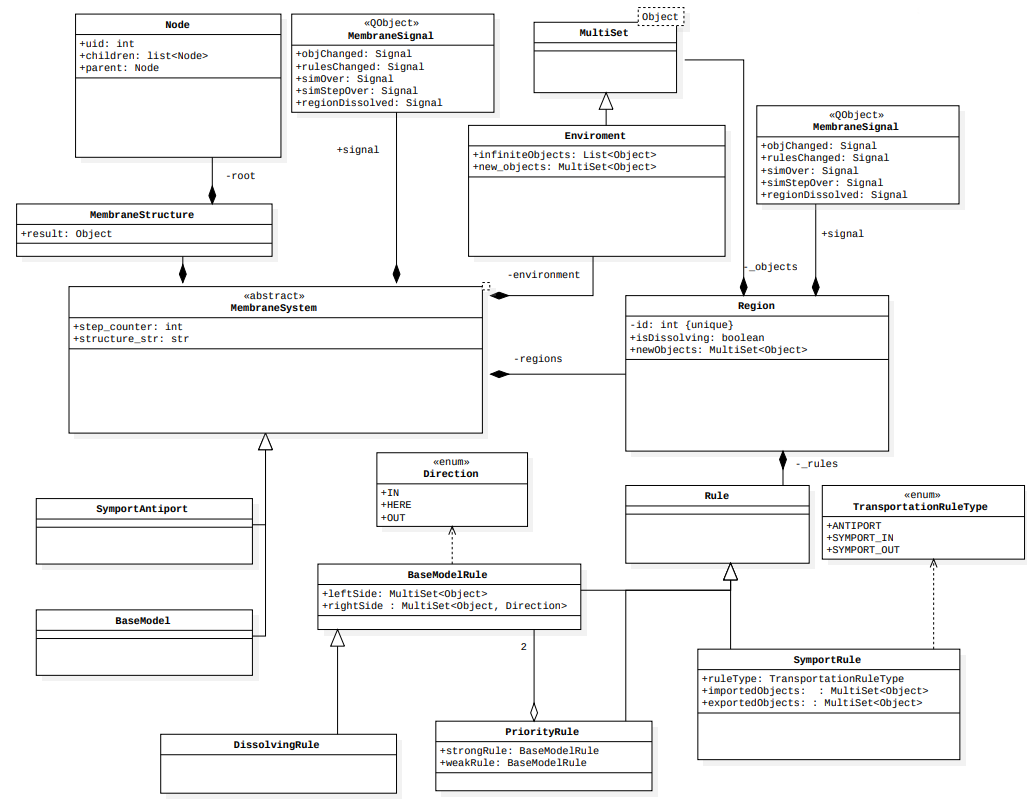
\includegraphics{model_uml_no_methods.png}}
	\caption{A modell osztály diagramja}
	\label{fig:model_no_methods}
\end{figure}

A \ref{fig:model_no_methods} ábra mutatja az osztály diagramot, amelyben még nem szerepelnek az osztályszintű-és példánymetódusok. Az eddig említett osztályokon felül megjelenik két, a modell és a nézet közötti üzenetváltásért felelős, \verb|QObject|-ből leszármazó osztály, a \verb|MembraneSignal| és a \verb|RegionSignal| . Az előbbi a teljes membránrendszerben előforduló jelzéseket küldi tovább majd a megjelenítésért felelős osztályoknak, míg az utóbbi az egyes régiók tartalmának megváltozását hivatott jelezni. A szoftver működéséhez szükséges objektumok meghatározása még nem elegendő céljának megvalósításához, ugyanis szükség van ezen osztályok metódusain keresztül a szimulálás folyamatának megtervezésére is.

\subsection{Objektumok}

Az objektumokat reprezentáló multihalmazokat a \verb|MultiSet| osztály segítségével hozhatjuk létre. Ezen osztály példányai felett értelmezve van az unió, kivonás művelete, a részhalmaz reláció, illetve lekérdezhető egy tetszőleges objektum multiplicitása. A \verb|MultiSet| osztály kiemelt fontosságú a számítás során, hiszen egy szabály alkalmazhatóságának eldöntéséhez két multihalmaz (nevezetesen a régió objektumait tartalmazó és a szabály bal oldala) közötti részhalmaz reláció eldöntésére van szükség. Ha valóban alkalmazható egy szabály, akkor a szabály bal oldala felhasználásra kerül, tehát egy kivonás műveletet kell végezni, a létrejövő objektumok pedig a megfelelő régióhoz az unió műveletével tudnak hozzákerülni. Tehát az osztályt nem csak a régiók, hanem a szabályok is felhasználják működésük során.

\begin{figure}[H]
\centering
	\scalebox{0.75}[0.75]{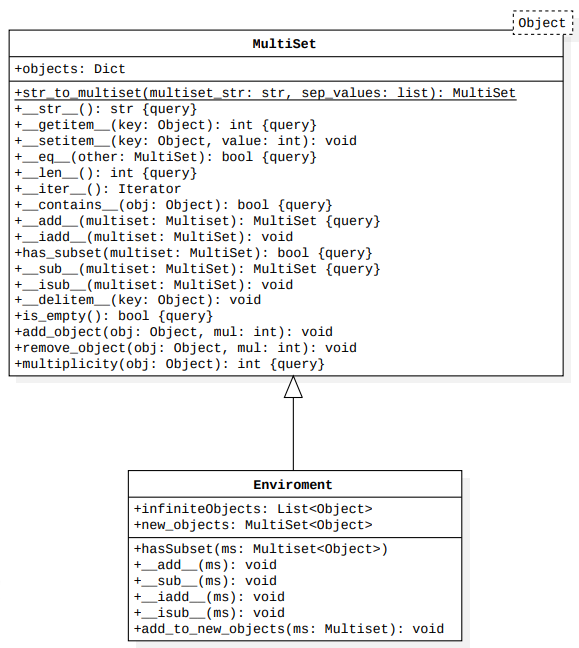
\includegraphics{multiset_class.png}}
	\caption{Az objektumokat reprezentáló multihalmaz és a környezet}
	\label{fig:multiset_uml}
\end{figure}

A környezet reprezentálására hivatott \verb|Environment| osztály a korlátlanul rendelkezésre álló objektumokat tartalmazó \verb|infinite_obj| listával egészíti ki a \verb|MultiSet| osztályt, illetve az ősosztályban használt műveletek is felüldefiniálja a helyes viselkedés érdekében. Mivel a környezet is \verb|MultiSet| típusú, ezért a dinamikus típusosság következtében az unió műveletet meghívhatnánk rá \verb|MultiSet| típusú paraméterrel, ennek eredménye szintén \verb|MultiSet| típusú lenne (ami a környezet aktualizálásakor egy evolúciós lépésben nem lenne szerencsés). Ennek elkerülése érdekében ezen műveleteket implementáció nélkül felüldefiniálja az osztályt és csak olyan műveletet biztosít, amely a metódushoz tartozó (\verb|this|)  példányhoz unió művelet segítségével hozzáad egy multihalmazt. A hozzáadás során az \verb|infinite_obj|-ban megtalálható objektumok figyelmen kívül hagyhatók. A kivonás esetén is hasonlóan járunk el, illetve ha speciálisan olyan objektumot kell levonni, amely korlátlan számban áll rendelkezésre, olyankor az mellékhatás nélkül végrehajtódhat.

\subsection{Membránstruktúra}

Mivel a membránrendszer struktúrája egyes típusok esetében módosulhat, ezért fontos, hogy a rendszer szerkezetét ne statikusan legyen tárolva, hanem a membránrendszer megkonstruálása után is dinamikusan tudjon változni.  Ezeket az elvárásoknak megfelelő \textit{n}-áris fát láncolt lista adatszerkezettel valósítom meg, amelynek fejelemét (fák esetén inkább gyökerét)  a \verb|MembraneStructure| osztály adattagként tárolja el. Minden csúcs egyedi azonosítóval rendelkezik, amely megegyezik a hozzátartozó régió címkéjével. Emellett minden csúcs számontartja a saját szülőjét, illetve gyermekeiből álló \verb|children| listát, amelyhez az \verb|add_child| metódussal lehet új elemet fűzni. Az osztály többi művelete \textit{getter} vagy \textit{setter} metódusként funkcionál.

\begin{figure}[H]
\centering
	\scalebox{0.75}[0.75]{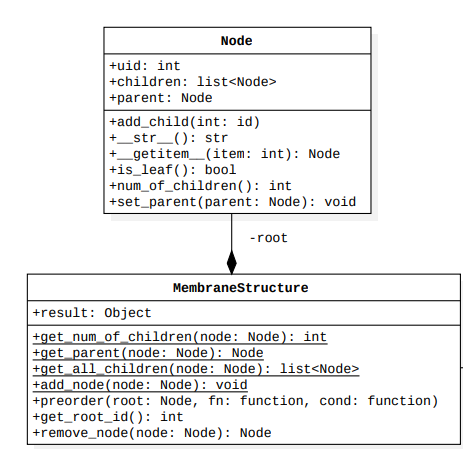
\includegraphics{node_and_structure_class.png}}
	\caption{A membránrendszer struktúrájáért felelős osztályok}
	\label{fig:node_and_structure_uml}
\end{figure}


A \verb|MembraneStructure| osztály a fa struktúra karbantartásáért és a struktúrával kapcsolatos ,,lekérdezésekért'' felelős. Ezen feladatok ellátásához kulcsszerepet kap a \verb|preorder(root, fn, cond)| metódus, amely a bejárja a fát és ha egy \textit{n} csúcsra teljesül a \verb|cond| függvény feltétele, akkor az  \verb|fn| függvény kerül meghívásra.

\lstset{caption={Membránstruktúra preorder bejárása}, label=src:py}
\begin{lstlisting}[language={Python}]
def preorder(self, root, fn, cond):
        if root is None:
            return
        if cond(root):
            self.result = fn(root)
        else:
            iter_count = root.num_of_children()
            for i in range(iter_count):
                self.preorder(root.children[i], fn, cond)
\end{lstlisting}

A \verb|MembraneStructure| kialakítása igazodik ehhez a szemantikához, mivel mind a négy osztályszintű metódus és a \verb|remove_node()| metódus is egy \textit{Node} típusú paramétert vár, amelyen végrehajtják a kívánt műveletet. Tehát ezen metódusok nem járják be a fát és keresik meg a megfelelő címkéjű csúcsot, hanem a \verb|preorder| függvény paramétereként kerülnek felhasználásra, amelyben a feltétel a csúcs egyedi azonosítójára szűr. Mivel a rekurzív függvénynek tetszőleges típusú visszatérési értéke lehetne, ezért a visszaadandó érték a struktúra \verb|result| adattagjába kerül. Az osztály felépítése garantálja, hogy a result lekérdezései nem keresztezhetik egymást, ezáltal elkerülve az inkonzisztens és helytelen értékeket.

\subsection{Szabályok}

A szabályok a membránrendszer számításaiban központi szerepet kapnak, ám kevés olyan tulajdonságuk van, amely minden típusban közös vonásként jelenik meg. Ezért az absztrakt \verb|Rule| ősosztály kevés implementálandó metódust határoz meg, csak a szabályhoz tartozó szöveges reprezentáció, illetve a szabály súlyát meghatározó műveletek meglétét követeli. 


\begin{figure}[H]
\centering
	\scalebox{0.6}[0.6]{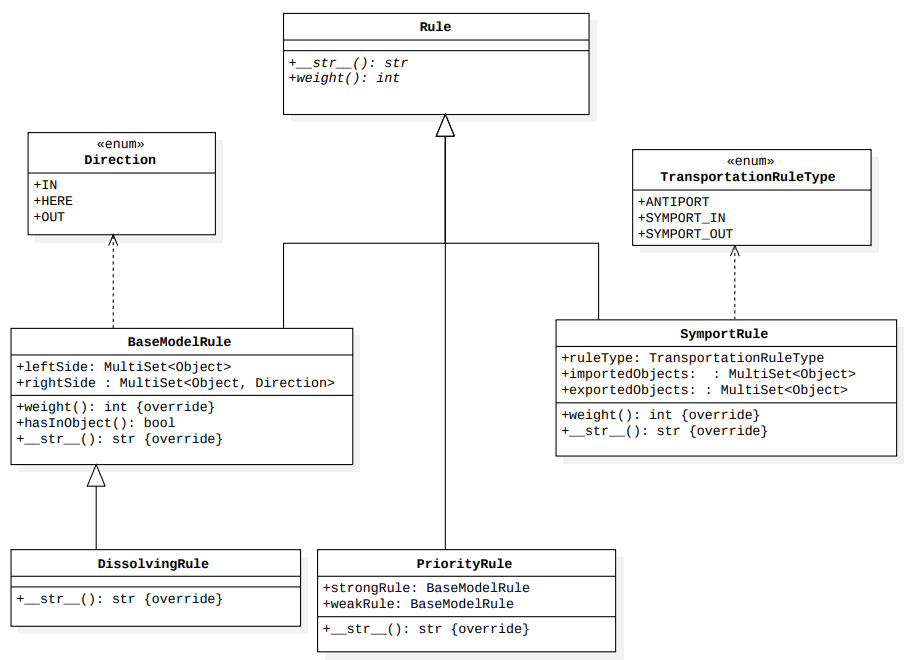
\includegraphics{uml_rule_class.png}}
	\caption{A membránrendszer szabályait modellező osztályok}
	\label{fig:rule_uml}
\end{figure}

Az alapmodellhez tartozó \verb|BaseModelRule| osztály a leszármazás mellett rögzíti a modellezéséhez szükséges két adattagot. Az egyik a \verb|left_side|, amely a szabály végbemeneteléhez szükséges objektumokból álló multihalmazt tárolja ( objektum-multiplicitás párok formájában), a másik pedig a \verb|right_side|, amely a szabály alkalmazásának következtében létrejövő objektumokat és azok mozgásának irányát adja meg. Ezen irányok jelzésére a \verb|Direction| osztályban rögzített \verb|HERE|, \verb|IN| és \verb|OUT| felsorolási típus értékei hivatottak. Tehát a \verb|right_side| olyan multihalmazban a megfelelő multiplicitással \verb|(objektum, irány)| párok szerepelnek.
Tehát egy evolúciós lépésben az alapmodellbeli szabály alkalmazhatóságának eldöntése a szabály bal oldala és a régióhoz tartozó objektumokból álló multihalmaz közötti tartalmazási reláció vizsgálatával ellenőrizhető. 
Az alapmodell kiegészítéseként beszélhetünk a feloldódás fogalmáról, amely a modellezés során a \verb|BaseModelRule|-ból leszármaztatott \verb|DissolvingRule| osztály segítségével kerül megvalósításra. Ez az osztály semmilyen új metódust vagy adattagot nem vesz fel, az információtartalom a példányosítása mögött rejlik, hiszen ilyen típusú szabály alkalmazása az adott régió \verb|is_dissolving| adattagjának igaz értékre billentését idézi elő. 
Az alapmodell másik ilyen kiterjesztése a szabályok közötti részbenrendezés lehetőségét nyújtja, amelyet az alkalmazás két szabály közötti prioritás rögzítésével támogatja. Az ilyen szabályok közötti relációk leírására a \verb|PriorityRule| szolgál, amely létrehozásakor két alapmodelli szabályt vár paraméterül.
Egy \verb|PriorityRule| típusú szabály alkalmazhatóságának vizsgálata során először a nagyobb prioritással rendelkezdő szabály alkalmazhatóságát kell vizsgálni, majd annak esetleges  sikertelensége esetén lehet a kisebb prioritással rendelkező szabály alkalmazhatóságát elemezni.


\subsection{Régiók}

\begin{figure}[H]
\centering
	\scalebox{0.6}[0.6]{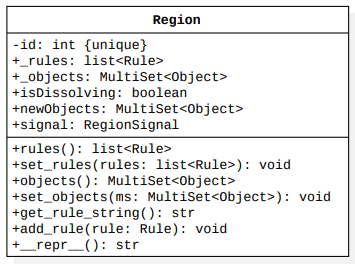
\includegraphics{uml_region_class.png}}
	\caption{A membránrendszer régióit reprezentáló osztály}
	\label{fig:region_uml}
\end{figure}

Egy régió azonosítására a saját egyedi azonosítóját (\verb|id|) használja az alkalmazás, amely megegyezik a membránstruktúrában a hozzá tartozó \verb|Node| objektum \verb|uid| adattagjában tárolt értékkel. Ez az érték a rendszer számítása során nem változik, egyedül egy régió szülőjének címkéje változhat meg (alapmodell esetén feloldódás következtében), ezért ezt az értéket nem lehet statikusan letárolni. A feloldódás jelzésére az \verb|is_dissolving| adattag hivatott, amelynek igaz értékre billenése esetén az evolúciós lépés végén a régió felbomlik. A régió emellett felveszi a \verb|new_objects| adattagot is, amely azon objektumok eltárolására szolgál, amelyek az éppen zajló evolúciós lépésben kerültek a régióba. Ez azért fontos, mert a maximális párhuzamosság elve szerinti szabályok kiválasztása egyidejűleg történik meg az ütem elején, tehát az egyik szabály alkalmazásának mellékhatása nem befolyásolhatja a kiválasztott szabályokat. Ezért amikor alkalmazásra kerül egy szabály, a jobb oldalán található objektumok elrejtésre kerülnek a további szabályok elől, majd az evolúciós lépésben a maximális szabálymultihalmaz után kerülnek a régió \verb|objects| multihalmazába. 

\subsection{Absztrakt membránrendszer és leszármazottai}

\subsection{Számítás algoritmusa}

\section{Forráskódok}

Nulla sodales purus id mi consequat, eu venenatis odio pharetra. Cras a arcu quam. Suspendisse augue risus, pulvinar a turpis et, commodo aliquet turpis. Nulla aliquam scelerisque mi eget pharetra. Mauris sed posuere elit, ac lobortis metus. Proin lacinia sit amet diam sed auctor. Nam viverra orci id sapien sollicitudin, a aliquam lacus suscipit. Quisque ac tincidunt leo \ref{src:cpp}. és \ref{src:csharp}.~forráskód:

\lstset{caption={Hello World in C++}, label=src:cpp}
\begin{lstlisting}[language={C++}]
#include <stdio>

int main() 
{
	int c;
	std::cout << "Hello World!" << std::endl;

	std::cout << "Press any key to exit." << std::endl;
	std::cin >> c;
	
	return 0;
}
\end{lstlisting}

\lstset{caption={Hello World in C\#}, label=src:csharp}
\begin{lstlisting}[language={[Sharp]C}]
using System;
namespace HelloWorld
{
	class Hello 
	{
		static void Main() 
		{
			Console.WriteLine("Hello World!");
			
			Console.WriteLine("Press any key to exit.");
			Console.ReadKey();
		}
	}
}
\end{lstlisting}

\subsection{Algoritmusok}

Az \ref{alg:ibb}.~algoritmus egy általános elágazás és korlátozás algoritmust (\emph{Branch and Bound algorithm}) mutat be. A \ref{step:selrule}.~lépésben egy megfelelő kiválasztási szabályt kell alkalmazni.
Példa forrása: \href{https://www.inf.u-szeged.hu/actacybernetica/}{Acta Cybernetica (ez egy hiperlink)}.

\begin{algorithm}[H]
\caption{A general interval B\&B algorithm}
\label{alg:ibb}
\textbf{\underline{Funct}} IBB($S,f$)
\begin{algorithmic}[1] % sorszámok megjelenítése minden n. sor előtt, most n = 1
\State Set the working list ${\cal L}_W$ := $\{S\}$ and the final list ${\cal L}_Q$ := $\{\}$
\While{( ${\cal L}_W \neq \emptyset$ )} \label{alg:igoend}
	\State Select an interval $X$ from ${\cal L}_W$ \label{step:selrule}\Comment{Selection rule}
	\State Compute $lbf(X)$ \Comment{Bounding rule}
	\If{$X$ cannot be eliminated} \Comment{Elimination rule}
		\State Divide $X$ into $X^j,\ j=1,\dots, p$, subintervals   \Comment{Division rule}
		\For{$j=1,\ldots,p$}
			\If{$X^j$ satisfies the termination criterion} \Comment{Termination rule}
				\State Store $X^j$ in ${\cal L}_W$
			\Else
				\State Store $X^j$ in ${\cal L}_W$
			\EndIf
		\EndFor
	\EndIf
\EndWhile
\State \textbf{return} ${\cal L}_Q$
\end{algorithmic}
\end{algorithm}
